% Encoding circuit U(x) of notebook 45d, Eq. (16), exactly as in `feature_circuit`, drawn for N = 4, d = 2, L = 2.
% One layer: H on every qubit; Rz(2 s xt_q) on every qubit with xt_q = x_1 (even q) or x_2 (odd q);
% Rzz(2 s^2 xt_q xt_{q+1}) = exp(-i s^2 x_1 x_2 Z_q Z_{q+1}) on the pairs (0,1), (1,2), (2,3), applied in this order.
% The layer is repeated L = 2 times.  The product encoding omits the Rzz gates.
\documentclass[tikz,border=6pt]{standalone}
\usepackage{amsmath,amssymb,bm}
\usetikzlibrary{arrows.meta,decorations.pathreplacing,calc,positioning}
\newcommand{\ket}[1]{\lvert #1\rangle}
\begin{document}
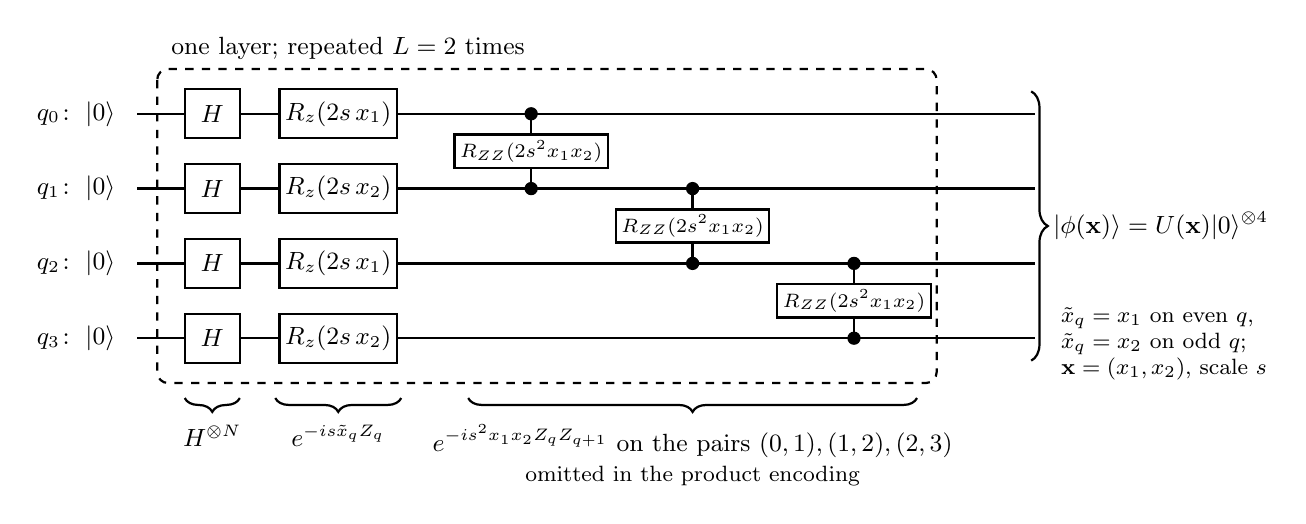
\begin{tikzpicture}[thick, >=Stealth, x=1cm, y=0.95cm,
    gate/.style={draw, fill=white, minimum height=0.62cm, minimum width=0.7cm, inner sep=2pt, font=\small},
    zz/.style={draw, fill=white, inner sep=2pt, font=\scriptsize}]
  % wires
  \foreach \q in {0,...,3} {
    \node[anchor=east, font=\small] at (-0.15,-\q) {$q_{\q}\!:\ \ket{0}$};
    \draw (0,-\q) -- (11.4,-\q);
  }
  % layer box
  \draw[dashed, rounded corners] (0.25,0.6) rectangle (10.15,-3.6);
  \node[font=\small, anchor=west] at (0.3,0.88) {one layer; repeated $L=2$ times};
  % Hadamards
  \foreach \q in {0,...,3} \node[gate] at (0.95,-\q) {$H$};
  % Rz with cyclic features
  \foreach \q/\f in {0/1, 1/2, 2/1, 3/2} \node[gate] at (2.55,-\q) {$R_z(2s\,x_{\f})$};
  % Rzz on neighbouring pairs, staggered as in the code (0,1) -> (1,2) -> (2,3)
  \newcommand{\zzgate}[3]{% x, q_i, q_j
    \fill (#1,-#2) circle (2.4pt); \fill (#1,-#3) circle (2.4pt);
    \draw (#1,-#2) -- (#1,-#3);
    \node[zz] at (#1,{-(#2+#3)/2}) {$R_{ZZ}(2s^2x_1x_2)$};}
  \zzgate{5.0}{0}{1}
  \zzgate{7.05}{1}{2}
  \zzgate{9.1}{2}{3}
  % braces
  \draw[decorate, decoration={brace, amplitude=5pt, mirror}] (0.6,-3.8) -- (1.3,-3.8)
       node[midway, below=6pt, font=\small] {$H^{\otimes N}$};
  \draw[decorate, decoration={brace, amplitude=5pt, mirror}] (1.75,-3.8) -- (3.35,-3.8)
       node[midway, below=6pt, font=\small, align=center] {$e^{-is\tilde x_qZ_q}$};
  \draw[decorate, decoration={brace, amplitude=5pt, mirror}] (4.2,-3.8) -- (9.9,-3.8)
       node[midway, below=6pt, font=\small, align=center] {$e^{-is^2x_1x_2Z_qZ_{q+1}}$ on the pairs $(0,1),(1,2),(2,3)$\\
       {\footnotesize omitted in the product encoding}};
  % output
  \node[font=\small, anchor=west] at (11.5,-1.5) {$\ket{\phi(\mathbf x)}=U(\mathbf x)\ket{0}^{\otimes 4}$};
  \draw[decorate, decoration={brace, amplitude=6pt}] (11.35,0.3) -- (11.35,-3.3);
  % feature assignment
  \node[font=\footnotesize, align=left, anchor=north west] at (11.6,-2.45)
       {$\tilde x_q=x_1$ on even $q$,\\ $\tilde x_q=x_2$ on odd $q$;\\ $\mathbf x=(x_1,x_2)$, scale $s$};
\end{tikzpicture}
\end{document}
